\documentclass[12pt]{exam}

\usepackage[latin1]{inputenc}
\usepackage{graphicx}
\usepackage[hidelinks]{hyperref}
\usepackage{float}
\usepackage{mathtools}
\usepackage{longtable}
\usepackage[numbers]{natbib}
\usepackage{amssymb}
\usepackage{tabularx}
\usepackage{tikz}
\usepackage{longtable}
\usepackage{ifthen}
\usepackage[margin=0.75in]{geometry}

\newcommand{\argmax}[1]{\underset{#1}{\operatorname{arg}\,\operatorname{max}}\;}
\newcommand{\argmin}[1]{\underset{#1}{\operatorname{arg}
\,\operatorname{min}}\;}

%Figures aliases
%Usage: \image{path}{width}{caption}{label}
%Try to allways use \image and let latex fix positioning of figures.
%By passing 'null' as width the latex will use the figures default size
%Do however but the command at the wanted position within the text, 
%if we at a later stage want to fix the positioning of all images it could be done by rewriting this alias.
\newcommand{\image}[4]{
	\ifthenelse{\equal{false}{true}}{%true - true => latex fixes positioning, mismatch => forced positioning by float
		\begin{figure}[ht]
			\centering
			\insertImage{#1}{#2}
			\caption{#3}
			\label{#4}
		\end{figure}
	}{
		\imageHere{#1}{#2}{#3}{#4}
	}	
}
\newcommand{\imageHere}[4]{
	\begin{figure}[H]
		\centering
		\insertImage{#1}{#2}
		\caption{#3}
		\label{#4}
	\end{figure}
}
%Helper function, do not use
\newcommand{\insertImage}[2]{
	\ifthenelse{\equal{#2}{null}}{
		\includegraphics{#1}
	}{
		\includegraphics[width=#2]{#1}
	}
}
\newcommand{\tcite}[1]{
	\citeauthor{#1} \citeyearpar{#1}
}

%%Force correct display style for math environments
\everymath{\displaystyle}
\begin{document}
	\chapter{PrePostTest}
\usetikzlibrary{quotes,angles,calc}
Which angle is bigger in each pair?

\begin{tikzpicture}[thick, scale= 2]
	\draw (0,0) -- (0:1);
	\draw (0,0) -- (80:1);
	\begin{scope}[shift={(2,0)}]
		\draw (0,0) -- (60:2);
		\draw (0,0) -- (20:2);
  \end{scope}
\end{tikzpicture}

\bigskip

\begin{tikzpicture}[thick, scale= 2]
	\draw (0,0) -- (45:1);
	\draw (0,0) -- (-45:1);
	\begin{scope}[shift={(2,0)}]
		\draw (0,0) -- (-45:1);
		\draw (0,0) -- (-135:1);
  \end{scope}
\end{tikzpicture}

\begin{tikzpicture}[thick, scale= 2]
	\draw (0,0) -- (60:1);
	\draw (0,0) -- (80:1);
	\begin{scope}[shift={(2,0)}]
		\draw (0,0) -- (40:1);
		\draw (0,0) -- (10:1);
  \end{scope}
\end{tikzpicture}

Find the missing measures of the angles (59 logo and geometry)

\begin{tikzpicture}
  \draw
  (3,-1) coordinate (a) node[right] {a}
  -- (0,0) coordinate (b) node[left] {b}
  -- (2,2) coordinate (c) node[above right] {c}
  pic["$\alpha$",draw=orange,<->,angle eccentricity=1.2,angle radius=1cm] {angle=a--b--c};
\end{tikzpicture}

\newcommand{\tikzAngleOfLine}{\tikz@AngleOfLine}                               
  \def\tikz@AngleOfLine(#1)(#2)#3{%                                            
  \pgfmathanglebetweenpoints{%                                                 
    \pgfpointanchor{#1}{center}}{%                                             
    \pgfpointanchor{#2}{center}}                                               
  \pgfmathsetmacro{#3}{\pgfmathresult}%                                        
  }                                                                            
\newcommand{\tikzMarkAngle}[3]{                                                
\tikzAngleOfLine#1#2{\AngleStart}                                              
\tikzAngleOfLine#1#3{\AngleEnd}                                                
\draw #1+(\AngleStart:0.15cm) arc (\AngleStart:\AngleEnd:0.15cm);              
}                                                                              

\begin{tikzpicture}[scale=4,line width=1pt]                                    
  \coordinate (A) at (0,0);                                                    
  \coordinate (B) at ($(A)+(90:1)$);                                                    
  \coordinate (C) at ($(B)+(-30:2)$);                                                
  \draw (A) -- (B) -- (C) -- cycle;                                            
	
  \tikzMarkAngle{(C)}{(B)}{(A)}   
	\node at ($(C)+(160:0.23)$) {?=\underline{\hspace{1cm}}};
	
	\tikzMarkAngle{(A)}{(B)}{(C)}
	\node at ($(A)+(45:0.23)$) {$90^\circ$};
	
	\tikzMarkAngle{(B)}{(A)}{(C)}           
	\node at ($(B)+(-60:0.23)$) {$60^\circ$};
\end{tikzpicture}  

\begin{tikzpicture}[scale=4,line width=1pt]                                    
  \coordinate (A) at (0,0);                                                    
  \coordinate (B) at ($(A)+(80:1)$);                                                    
  \coordinate (D) at ($(A)+(0:3)$);                                                
	\coordinate (C) at ($(D)+(100:1.5)$);
  \draw (A) -- (B) -- (C) -- (D) -- cycle;                                            
	
  \tikzMarkAngle{(A)}{(B)}{(D)}   
	
	\tikzMarkAngle{(C)}{(B)}{(D)}           
	
	\tikzMarkAngle{(D)}{(A)}{(C)}          
	
	\draw[shift={(B)}] (-100:0.15cm) arc (-100:10:0.15cm);
\end{tikzpicture}  

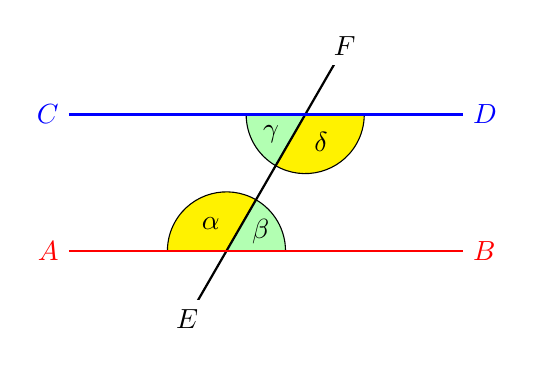
\begin{tikzpicture}
  \draw[fill=yellow] (0,0) -- (60:.75cm) arc (60:180:.75cm);
  \draw(120:0.4cm) node {$\alpha$};

  \draw[fill=green!30] (0,0) -- (right:.75cm) arc (0:60:.75cm);
  \draw(30:0.5cm) node {$\beta$};

  \begin{scope}[shift={(60:2cm)}]
    \draw[fill=green!30] (0,0) -- (180:.75cm) arc (180:240:.75cm);
    \draw (30:-0.5cm) node {$\gamma$};

    \draw[fill=yellow] (0,0) -- (240:.75cm) arc (240:360:.75cm);
    \draw (-60:0.4cm) node {$\delta$};
  \end{scope}

  \begin{scope}[thick]
    \draw (60:-1cm) node[fill=white] {$E$} -- (60:3cm) node[fill=white] {$F$};
    \draw[red]                   (-2,0) node[left] {$A$} -- (3,0) 
                                        node[right]{$B$};
    \draw[blue,shift={(60:2cm)}] (-3,0) node[left] {$C$} -- (2,0) 
                                        node[right]{$D$};
  \end{scope}
\end{tikzpicture}

Estimate the angles

\begin{tikzpicture}[scale=4,line width=1pt]                                    
  \coordinate (A) at (0,0);                                                    
  \coordinate (B) at ($(A)+(90:1)$);                                                    
  \coordinate (C) at ($(A)+(30:1)$);                                                
  \draw (A) -- (B);                                            
	\draw (A) -- (C);                                            
  \tikzMarkAngle{(A)}{(B)}{(C)}   
\end{tikzpicture}  

\begin{tikzpicture}[scale=4,line width=1pt]                                    
  \coordinate (A) at (0,0);                                                    
  \coordinate (B) at ($(A)+(90:1)$);                                                    
  \coordinate (C) at ($(A)+(0:1)$);                                                
  \draw (A) -- (B);                                            
	\draw (A) -- (C);                                            
  \tikzMarkAngle{(A)}{(B)}{(C)}   
\end{tikzpicture}  

\begin{tikzpicture}[scale=4,line width=1pt]                                    
  \coordinate (A) at (0,0);                                                    
  \coordinate (B) at ($(A)+(120:1)$);                                                    
  \coordinate (C) at ($(A)+(0:1)$);                                                
  \draw (A) -- (B);                                            
	\draw (A) -- (C);                                            
  \tikzMarkAngle{(A)}{(B)}{(C)}   
\end{tikzpicture}  

\begin{tikzpicture}[scale=4,line width=1pt]                                    
  \coordinate (A) at (0,0);                                                    
  \coordinate (B) at ($(A)+(-90:1)$);                                                    
  \coordinate (C) at ($(A)+(-135:1)$);                                                
  \draw (A) -- (B);                                            
	\draw (A) -- (C);                                            
  \tikzMarkAngle{(A)}{(B)}{(C)}   
\end{tikzpicture}  

\begin{tikzpicture}[scale=4,line width=1pt]                                    
  \coordinate (A) at (0,0);                                                    
  \coordinate (B) at ($(A)+(0:1)$);                                                    
  \coordinate (C) at ($(A)+(180:1)$);                                                
  \draw (A) -- (B);                                            
	\draw (A) -- (C);                                            
  \tikzMarkAngle{(A)}{(B)}{(C)}   
\end{tikzpicture}  

%parallelogram
\begin{tikzpicture}[scale=4,line width=1pt]                                    
  \coordinate (A) at (0,0);                                                    
  \coordinate (B) at (2,0);                                                    
  \coordinate (C) at ($(B)+(150:1)$);                                                
	\coordinate (D) at ($(A)+(150:1)$);                                                
  \draw (A) -- (B) -- (C) -- (D) -- cycle;                                            
	
  \tikzMarkAngle{(A)}{(B)}{(D)}   
	
	\tikzMarkAngle{(B)}{(A)}{(C)}
	
	\tikzMarkAngle{(C)}{(B)}{(D)}           
	\draw[shift={(D)}] (-30:0.15cm) arc (-30:0:0.15cm);      
\end{tikzpicture}  
	\begin{center}
		\Huge{TurtleBot}
	\end{center}

	\section{The TurtleBot application}
	The \textit{graphics view} seen in figure~\ref{fig:augmented} is the first thing you'll see when the application starts. 
	In order for you to get familiar with the layout we have highlighted the different components, 
	and provided a simple description of them below figure~\ref{fig:augmented}. 
	\image{imgs/SimpleMainAugmented.png}{\columnwidth}{Graphics view}{fig:augmented}
	
	\begin{description}
		\item[1] This is the available \textit{codeblocks} for your \textit{program}.
		\item[2] The \textit{startblock}. This is a special kind of \textit{codeblock}. 
			It may not be moved or removed, and must always be the first \textit{codeblock} in the \textit{program}.
		\item[3] The \textit{program}. This part consists of one of more \textit{codeblocks}, and are the part which tells the robot what to do.
			An explaination of the different codeblocks can be seen in section~\ref{sec:normal} and section~\ref{sec:extended}.
		\item[4] The \textit{Options} menu. 
		\item[5] The \textit{Run} button. Pressing this button run the \textit{program}.
		\item[6] The \textit{Clear} button. This button will remove all blocks except the \textit{startblock}.
		\item[7] The \textit{Input mode} button. This button will change the input view. 
		If you are working in the \textit{graphics view} it will change to the \textit{textual view}, and vise versa.
	\end{description}
	
	\subsection{Views}
	The application is divided into several different views and panels. 
	When you first start the application it will start in the \textit{graphics view}(see figure~\ref{fig:augmented}), 
	this is the view where most of the programming will be done. Programming in this view is done by dragging \textit{codeblocks} around the screen.
	As an alternative to the \textit{graphics view}, there is also a \textit{textual view}(see figure~\ref{fig:extendedTextual}). 
	The \textit{textual view} has the same function and goal as the \textit{graphics view}, but requires you to write the code yourselves in text form.
	Changing between \textit{graphics view} and \textit{textual view} can be done by pressing the button numbered \textbf{7} in figure \ref{fig:augmented}. 
	Any \textit{code} or \textit{codeblocks} are then converted to the correct format.
	
	\subsubsection{Graphics view}
	In order to create program you drag the codeblock you want from the available blocks down to the startblock, a small indicator should appear.
	In order to change the order of your codeblocks, simply drag the codeblock you want to move into the correct position. 
	If you want to remove a codeblock from your program just drag it back to the list of available blocks at the top.
	
	\subsubsection{Textual view}
	When working in \textit{textual view} you must write the code yourselves. 
	In figure~\ref{fig:extendedTextual} you see an example of a \textit{program} written with in \textit{extened mode}.
		
	\subsection{Normal mode}\label{sec:normal}
	When starting the application for the first time, it will start in what is called \textit{normal mode} showing the \textit{graphics view}.
	In \textit{normal mode} you have four \textit{codeblocks} available to you: 
	
	\begin{center}
		\begin{tabular}{ll}
			\textbf{FWD - Forward} & \textbf{BACK - Backward}\\
			\textbf{TL - Turn Left} & \textbf{TR - Turn Right}\\
			\label{tab:moves}
		\end{tabular}
	\end{center}
	
	\noindent
	\textbf{FWD} and \textbf{BACK} makes the robot move forward and backward respectively. The input value determines how far the robot will go.
	\textbf{TL} and \textbf{TR} makes the robot turn either left of right. The input value determines how many degrees it will turn. 
	
	\bigskip\noindent
	In figure~\ref{fig:augmented} you can see an example where all these four \textit{codeblocks} are used. 
	The resulting picture from this \textit{program} can be seen in figure~\ref{fig:simpleProg}.
	\image{imgs/SimpleProg.PNG}{null}{The result from running the program in figure~\ref{fig:augmented}}{fig:simpleProg}
	
	\subsection{Extended mode}\label{sec:extended}
	If \textit{extended mode} is turn on you will see five new \textit{codeblocks} appear as available (figure~\ref{fig:extendedMain}).
	These blocks are related to programs that need \textit{variables}, \textit{procedures} and \textit{loops}. 
	The usage of these blocks and how they work will be explained in another document.
	
	\image{imgs/ExtendedMain.PNG}{0.7\columnwidth}{The main view when extended mode is on.}{fig:extendedMain}
	\image{imgs/ExtendedTextual.PNG}{0.7\columnwidth}{The textual view when extended mode is on.}{fig:extendedTextual}
	\subsection{The simulator}
	The \textit{simulator view} is to show you the result of your program. 
	This view shows when you press the \textbf{run} button(numbered 5 in figure~\ref{fig:augmented}). 
	When the simulation is running you have the ability to stop it by pressing the \textbf{run} button (turned red), 
	or by pressing the \textbf{change view} button(numbered 7 in figure~\ref{fig:augmented}).
	\image{imgs/Simulator.PNG}{0.7\columnwidth}{The simulator view.}{fig:simulator}
	
	\subsection{Options}
	The \textit{options panel} allows you to change the behaviour of the application at runtime, change the inital setup, and connect to an external robot.
	The yellow \textit{Connect} button is only visible if the device has bluetooth enabled. 
	
	\bigskip\noindent
	To connect to an external robot; click on the \textit{Connect} button and wait for a list of robots to show up on the screen(figure~\ref{fig:connectionSelection}),
	click on the desired robot and wait for the connection to happen. If everything works fine the \textit{Connect} button should turn green, this is an indication that
	the application is in contact with the robot.
	\image{imgs/Options.PNG}{0.7\columnwidth}{The options view.}{fig:options}
	\image{imgs/ConnectionSelection.PNG}{0.7\columnwidth}{The list of available robots.}{fig:connectionSelection}
	\image{imgs/Connected.PNG}{0.7\columnwidth}{The options view when connected to a robot.}{fig:optionsConnected}
	\subsubsection{OnScreen keyboard}
	This is fallback solution, if the native keyboard doesn't work.
	\image{imgs/Keyboard.PNG}{0.7\columnwidth}{The on screen keyboard for numeric input.}{fig:keyboardNumeric}
	\image{imgs/KeyboardAlpha.PNG}{0.7\columnwidth}{The on screen keyboard for alphanumeric input.}{fig:keyboardAlpha}
\end{document}

